\chapter{Developer documentation} % Developer guide
\label{ch:impl}

This chapter will cover the basics and the process of developing the Clang Static Analyzer checker. The developer is presumed to have the advanced knowledge of C++, the user experience of Linux, and familiarity with some of the build systems.


\section{Prerequisites}

Before writing the code, the developer must have a few necessary tools.


\begin{itemize}
    \item LLVM repository, available from GitHub \cite{llvm-project}
    \item Git version control system \cite{git}
    \item CMake
    \item Ninja build system. Other build systems can be used as well, however most LLVM developers use ninja 
    \item Development environment of your choice. VS Code, vim, CLion are viable options among others
\end{itemize}


\section{Building Clang} \label{build-clang}

The first step is to checkout LLVM repository from GitHub and create \emph{build}
directory inside. CMake is used to generate build files, it takes few parameters, which are self-explanatory. We use Ninja to start the build process and lastly, it is always a good idea to run all the tests before we start the development process.

\lstset{caption={}, label=build-llvm}
\begin{lstlisting}[language={bash}]
git clone https://github.com/llvm/llvm-project.git

cd llvm-project
mkdir build
cd build

# Configure build using cmake
cmake \
      -G "Ninja" \
      -DLLVM_ENABLE_PROJECTS="llvm;clang;clang-tools-extra" \
      -DCMAKE_BUILD_TYPE=RelWithDebInfo \
      -DBUILD_SHARED_LIBS=ON \
      -DLLVM_TARGETS_TO_BUILD=X86 \
      -DCMAKE_EXPORT_COMPILE_COMMANDS=ON \
      -DLLVM_ENABLE_ASSERTIONS=ON \
      ../llvm/

# -j 4 is number of parallel jobs
# It will take a while...
ninja -j 4

# Run all the tests
ninja check-all -j 4

# For ease of use user can add built binaries to the PATH
# export PATH="path/to/llvm-project/build/bin:$PATH"
\end{lstlisting}

The above steps will build clang along with some useful tools for development and testing. Later on, it is enough to rebuild just clang using \lstinline{ninja clang -j 4} while running only clang analysis specific tests is possible with \lstinline{ninja check-clang-analysis}


\section{Clang Static Analyzer Basics}
 
\subsection{Exploded Graph}
Static Analysis starts with reading plain source code, which is later transformed to Abstract Syntax Tree by Clang. Clang-Tidy, another LLVM native static analyzer tool, is using AST to find bugs in a source code, however, Clang SA takes a different approach and dives into Control Flaw Graph. Clang's CFG is a data structure that consists of AST statements, which are ordered as they are actually executed (figure \ref{fig:ast-and-cfg}). CFG is used by Clang to produce some compiler warnings, but Static Analyzer goes one step further and produces a new data structure called Exploded Graph. It essentially represents the result of the analysis, hence Clang Static Analyzer can be seen as a converter from AST to the Exploded Graph. Finding a bug in the source code is reduced to solving the graph reachability problem.

Exploded Graph consists of paths through CFG. Nodes are pairs of Program Point (the point between two statements, i.e. we finished the first but haven't started evaluating the second) and Program State (the big picture: how already evaluated statements affected the analysis).


\begin{figure}[H]
	\centering
	\subfigure[AST and CFG of x + y + z]{
		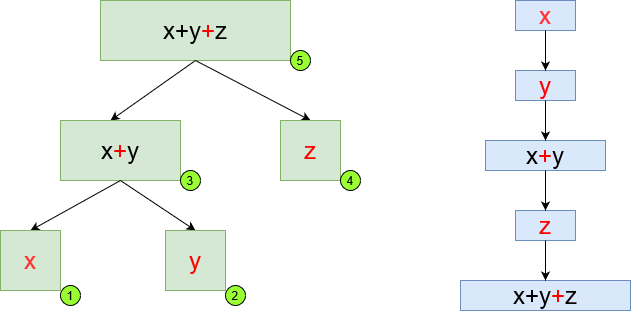
\includegraphics[width=\textwidth]{images/CFG_AST.png}}
	\hspace{30pt}
	\subfigure[AST and CFG of x ? y : z]{
		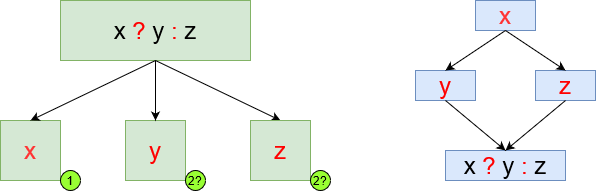
\includegraphics[width=\textwidth]{images/CFG_AST2.png}}
	\caption{Comparison of AST and CFG}
	\label{fig:ast-and-cfg}
\end{figure}

\subsection{Checkers}
Checkers are independent analyzer modules. They inherit from a template class \lstinline{Checker}; the template parameters are types of events to which checker is subscribed. For example, if a checker is interested in an event that occurs after a function call is processed, it can inherit from \lstinline{Checker<check::PostCall>} and implement \lstinline{checkPostCall} to inspect the event, issue a warning if necessary, or provide additional information to the analysis (checkers are active participants in the graph building process). The Checker Developer's Guide \cite{noqa} contains a list of all such callbacks as well as examples of their use. 

\subsection{Custom Program States} \label{checker-states}
During the analysis there is no guarantee about the order in which the program will be explored, or even that all possible paths will be explored; As a result, when checkers need to keep track of information specific to their work, it can not be stored within a single checker class. Instead, they add the data to \lstinline{ProgramState}. There are few macros designed for this purpose:

\begin{itemize}
    \item \lstinline{REGISTER_TRAIT_WITH_PROGRAMSTATE} -- Used when the state information is a single value.
    \item \lstinline{REGISTER_LIST_WITH_PROGRAMSTATE} -- Used when the state information is a list of values.
    \item \lstinline{REGISTER_SET_WITH_PROGRAMSTATE} -- Used when the state information is a set of values.
    \item \lstinline{REGISTER_MAP_WITH_PROGRAMSTATE} -- Used when the state information is a map from a key to a value.
\end{itemize}

All the above data structures come with convenient getter and setter functions. However, since \lstinline{ProgramState} is immutable, whenever we modify the data inside it, a copy of the state with the change applied is created. By calling the \lstinline{CheckerContext::addTransition} function, the updated state must be returned to the analyzer core. 

\section{Implementation}
This section describes the implementation of alpha.security.cert.pos.34c and alpha.security.cert.env.InvalidPtr checkers. 

\subsection{alpha.security.cert.pos.34c} \label{putenv}

The idea behind this checker is straightforward, and as one of the LLVM reviewers put it, "the source code reads so easily, we might as well put it as the official CERT rule description".
We subscribe for function call events, determine if it is \lstinline{putenv}, and inspect its argument, see figure \ref{fig:putenv-diag}.


\begin{figure}[H]
	\centering
	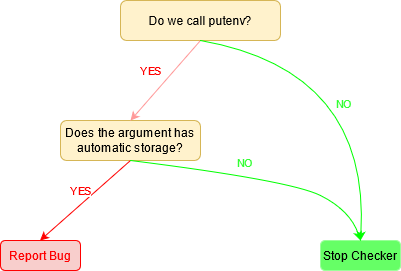
\includegraphics[]{images/putenv_diagram.png}
	\caption{PutenvWithAuto checker logic}
	\label{fig:putenv-diag}
\end{figure}

We use \lstinline{void checkPostCall(const CallEvent &Call, CheckerContext &C)} callback, which passes control to the checker after any function call.

\lstinline{CallEvent::isCalled()} function takes \lstinline{CallDescription} type as an argument and determines whether the called function matches one in the argument. To accomplish this, we first represent \lstinline{putenv} as \lstinline{CallDescription}.

\lstset{caption={}}
\begin{lstlisting}[language={C++}]
class PutenvWithAutoChecker : public Checker<check::PostCall> {
private:
    // ...
    const CallDescription Putenv{"putenv", 1};
public:
  void checkPostCall(const CallEvent &Call, CheckerContext &C) const;
};
void PutenvWithAutoChecker::checkPostCall(const CallEvent &Call,
                                          CheckerContext &C) const {
    if (!Call.isCalled(Putenv))
        return;                                      
    // ...
}
\end{lstlisting}

If the called function matches \lstinline{putenv}, we proceed to the argument, which is represented as \lstinline{SVal}.
We find the \emph{Memory Space Region} of this \lstinline{SVal} and compare it to the \lstinline{StackSpaceRegion}, the base class of everything stored on a stack.

\lstset{caption={}}
\begin{lstlisting}[language={C++}]
void PutenvWithAutoChecker::checkPostCall(const CallEvent &Call,
                                          CheckerContext &C) const {
    // ...
    SVal ArgV = Call.getArgSVal(0);
    const MemSpaceRegion *MSR = 
                    ArgV.getAsRegion()->getMemorySpace();
    if (!isa<StackSpaceRegion>(MSR))
        return;
    // ...
}
\end{lstlisting}

If we passed the both return statements in the preceding code snippets, we have violated POS34-C, as described in section \ref{rules}, and we must report the bug.

This is accomplished by creating \lstinline{PathSensitiveBugReport}, which takes three parameters:

\begin{enumerate}
    \item The type of a bug, instance of \lstinline{BugReport} class.
    \item Short descriptive error message.
    \item \lstinline{ExplodedNode}, the context in which the problem happened. This includes the location of the bug and the current state.
\end{enumerate}

After \lstinline{BugReport} is created, it must be passed to the analyzer core by \lstinline{CheckerContext::emitReport} function.

\lstset{caption={}}
\begin{lstlisting}[language={C++}]
class PutenvWithAutoChecker : public Checker<check::PostCall> {
private:
    BugType BT{this, "'putenv' function should not be called with auto variables", categories::SecurityError};
    // ...
};

void PutenvWithAutoChecker::checkPostCall(const CallEvent &Call,
                                          CheckerContext &C) const {
    // ...
    StringRef ErrorMsg = "The 'putenv' function should not be called with arguments that have automatic storage";
    ExplodedNode *N = C.generateErrorNode();
    auto Report = std::make_unique<PathSensitiveBugReport>(BT, ErrorMsg, N);
    C.emitReport(std::move(Report));
}
\end{lstlisting}

As a next step, we register the new checker by including two boilerplate functions to the source code: 
\lstset{caption={}}
\begin{lstlisting}[language={C++}]
void ento::registerPutenvWithAuto(CheckerManager &Mgr) {
  Mgr.registerChecker<PutenvWithAutoChecker>();
}

bool ento::shouldRegisterPutenvWithAuto(const LangOptions &) { 
    return true; 
}
\end{lstlisting}

By adding it to \lstinline{lib/StaticAnalyzer/Checkers/CMakeLists.txt}, the source code file is made visible to CMake.


Finally, inside \lstinline{include/clang/StaticAnalyzer/Checkers/Checkers.td} we select a package for the checker. The "CERT" package was created as a child of "SecurityAlpha," and it has two children, "POS" and "ENV" for our two checkers, respectively, as shown in the figure \ref{fig:packages}. One can verify that new checker was added by checking available checkers: \lstinline{clang -cc1 -analyzer-checker-help}.


\begin{figure}[H]
	\centering
	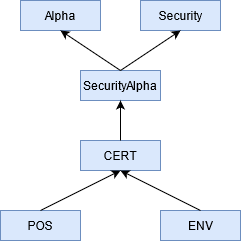
\includegraphics[]{images/packages.png}
	\caption{Checker packages tree}
	\label{fig:packages}
\end{figure}


\subsection{alpha.security.cert.env.InvalidPtr} \label{invalidptr}
A close examination of rules ENV31-C in section \ref{env31} and ENV34-C in section \ref{env34} reveals that they are very similar.
In both cases, some sequence of events invalidates pointers, and subsequent dereference of these invalid pointers results in unintended behavior. Furthermore, there are several scenarios in which a pointer escapes analysis, such as when it is passed to a function that cannot be analyzed. To further reduce false negatives we will add one more heuristic and issue a warning when an invalidated pointer is used as an argument to a function that is not conservatively evaluated. 

Assuming we have a collection of invalidated pointers, we can use the same logic to check for usage and issue a warning in both cases, as shown in figure \ref{fig:invalidptr}. This inspires us to create a single checker that handles both rules. 

\begin{figure}[H]
	\centering
	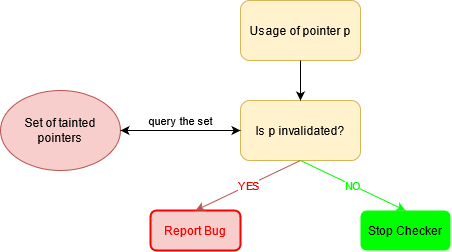
\includegraphics[]{images/invalid_ptr.png}
	\caption{High level logic of InvalidPtr checker}
	\label{fig:invalidptr}
\end{figure}


\subsubsection{Invalidating pointer -- ENV31-C} \label{invalidate-env31}
The first step is to get the \lstinline{envp} argument of \lstinline{main}, if it exists. For this we use \lstinline{checkBeginFunction}, which is called when the core begins to analyze a function. We check if function is \lstinline{main} and store third argument inside the state.

\lstset{caption={}}
\begin{lstlisting}[language={C++}]
// Stores the region of the environment pointer of 'main' (if present).
// Note: This pointer has type 'const MemRegion *'
REGISTER_TRAIT_WITH_PROGRAMSTATE(EnvPtrRegion, const void *)

void InvalidPtrChecker::checkBeginFunction(CheckerContext &C) const {
  if (!C.inTopFrame())
    return;

  const auto *FD = dyn_cast<FunctionDecl>(C.getLocationContext()->getDecl());
  if (!FD || FD->param_size() != 3 || !FD->isMain())
    return;

  ProgramStateRef State = C.getState();
  const MemRegion *EnvpReg =
      State->getRegion(FD->parameters()[2], C.getLocationContext());

  // Save the memory region pointed by the environment pointer
  State = State->set<EnvPtrRegion>(
      reinterpret_cast<void *>(const_cast<MemRegion *>(EnvpReg)));
  C.addTransition(State);
}
\end{lstlisting}

The next step is to move the \lstinline{envp} pointer to an invalidated set, if an environment modifying function is called,
Such functions are stored in \lstinline{CallDescriptionMap}, which is a map from \lstinline{CallDescription} to their handler functions.
Similarly to POS34-C, we use \lstinline{checkPostCall} to listen for function calls and, if it is found in our map, we call the handler. 


\lstset{caption={}}
\begin{lstlisting}[language={C++}]
  void EnvpInvalidatingCall(const CallEvent &Call, CheckerContext &C) const;
  using HandlerFn = void (InvalidPtrChecker::*)(const CallEvent &Call, CheckerContext &C) const;
  const CallDescriptionMap<HandlerFn> EnvpInvalidatingFunctions = {
      {{"setenv", 3}, &InvalidPtrChecker::EnvpInvalidatingCall},
      {{"unsetenv", 1}, &InvalidPtrChecker::EnvpInvalidatingCall},
      {{"putenv", 1}, &InvalidPtrChecker::EnvpInvalidatingCall},
      {{"_putenv_s", 2}, &InvalidPtrChecker::EnvpInvalidatingCall},
      {{"_wputenv_s", 2}, &InvalidPtrChecker::EnvpInvalidatingCall},
  };
  
  void InvalidPtrChecker::checkPostCall(const CallEvent &Call, CheckerContext &C) const {
    // Check if function invalidates 'envp' argument of 'main'
    if (const auto *Handler = EnvpInvalidatingFunctions.lookup(Call))
      (this->**Handler)(Call, C);
    // ...
  }
  
  void InvalidPtrChecker::EnvpInvalidatingCall(const CallEvent &Call, CheckerContext &C) const {
    // check if EnvPtrRegion exists
    // add it to the set of invalidated pointers
  }
\end{lstlisting}

\subsubsection{Invalidating pointer -- ENV34-C}

Aside from the five functions mentioned in the rule, many non-reentrant C library functions suffer from a similar problem.
This part of the checker was designed with genericness in mind, so that simply adding a new entry to the \lstinline{CallDescriptionMap} is sufficient to extend the checker. 


\lstset{caption={}}
\begin{lstlisting}[language={C++}]
  const CallDescriptionMap<EvalFn> PreviousCallInvalidatingFunctions = {
      {{"getenv", 1}, &InvalidPtrChecker::evalGetenv},
      {{"setlocale", 2}, &InvalidPtrChecker::evalSetlocale},
      {{"strerror", 1}, &InvalidPtrChecker::evalStrerror},
      {{"localeconv", 0}, &InvalidPtrChecker::evalLocaleconv},
      {{"asctime", 1}, &InvalidPtrChecker::evalAsctime},
  };
\end{lstlisting}

We create a custom map in which the keys are function names and the values are the results of the most recent call to this function: \\
\lstinline{REGISTER_MAP_WITH_PROGRAMSTATE(PreviousCallResultMap, const char *, const MemRegion *)} \\

On each call to the problematic function, we move the previous value (if it exists) from \lstinline{PreviousCallResultMap} to the invalidated set and update the map with the new memory region. 

\subsubsection{Reporting a bug}

Every time a specific memory location is accessed, the \lstinline{checkLocation} callback is triggered. Inside it we check if accessed memory is invalidated and report dereference of an invalidated pointer if it is. \\



\lstset{caption={}}
\begin{lstlisting}[language={C++}]
  void InvalidPtrChecker::checkLocation(SVal Loc, bool isLoad, const Stmt *S,
                                      CheckerContext &C) const {
  ProgramStateRef State = C.getState();

  // Ignore memory operations involving 'non-invalidated' locations.
  const MemRegion *InvalidatedSymbolicBase =
      findInvalidatedSymbolicBase(State, Loc.getAsRegion());
  if (!InvalidatedSymbolicBase)
    return;

  ExplodedNode *ErrorNode = C.generateNonFatalErrorNode();
  if (!ErrorNode)
    return;

  auto Report = std::make_unique<PathSensitiveBugReport>(
      BT, "dereferencing an invalid pointer", ErrorNode);
  C.emitReport(std::move(Report));
}
\end{lstlisting}

We also issue a warning whenever an invalidated pointer is passed as an argument to a non-conservatively analyzed function, as mentioned in \ref{invalidptr}.
We do this within \lstinline{checkPostCall} by traversing the array of arguments of a function and querying \lstinline{InvalidatedPointerSet} for each of them. 


% TODO
% \subsubsection{Path Diagnostics}
% To make the reports user friendly, custom visitor is implemented, which traverses the graph in search of invalidating function call and adds notes at the point of invalidation. 

% Next step is to make the report user friendly by adding notes, just like in figure \ref{fig:pos34termin2}. For POS34 we relied on built in \lstinline{bugreporter::trackExpressionValue()} for generating such a notes for the problematic \lstinline{putenv} argument, however for InvalidPtr we have to do it manually by creating   



\section{Testing}

Clang Static Analyzer checker testing consists of two parts: lit testing (see \ref{lit}) and running analysis on large code bases to find real world bug examples and, more importantly, to see if the analyzer breaks (see \ref{codebases}). 

\subsection{Lit} \label{lit}

The idea behind lit testing is simple: we create test files with faulty source code and specify which lines should generate a warning or a note.
Clang's \lstinline{-verify} flag performs this type of verification.
Consider the following example: 

\lstset{caption={}}
\begin{lstlisting}[language={C++}]
void getenv_test() {
  char *p1, *p2, *p3;

  p1 = getenv("VAR1");
  *p1; // no-warning

  p1 = getenv("VAR2"); // expected-note{{previous function call was here}}
  p3 = getenv("VAR3"); // expected-note{{'getenv' call may invalidate the the result of the previous 'getenv'}}

  p2 = getenv("VAR4");

  *p1; // expected-warning{{dereferencing an invalid pointer}}
}
\end{lstlisting}

Compliant code must also be tested; typically, a "no-warning" comment is written on lines that may be problematic; however, this is just a convention among analyzer developers and has no actual meaning behind it. 

\lstinline{expected-note} and \lstinline{expected-warning} are sometimes referred as verify comments. It is also possible to pass them some optional arguments, such as the distance between the comment and the actual warning, or the number of times the analyzer should throw an error.
For a better illustration, consider the following slightly modified version of the preceding example: 

\begin{lstlisting}[language={C++}]
void getenv_test1() {
  char *p1, *p2, *p3;

  p1 = getenv("VAR1");
  *p1; // no-warning

  p1 = getenv("VAR2");
  // expected-note@-1{{previous function call was here}}
  p3 = getenv("VAR3");
  // expected-note@-1{{'getenv' call may invalidate the the result of the previous 'getenv'}}

  p2 = getenv("VAR4");
  
  // expected-note@+1{{dereferencing an invalid pointer}}
  *p;
  // expected-warning@-1{{dereferencing an invalid pointer}}
}

\end{lstlisting}

\subsubsection{LLVM Integrated Tester}
llvm-lit is a lightweight tool for LLVM black box testing.

Each lit test file should begin with the following comment:
\lstinline{// RUN: <command>}, where command is argument for llvm-lit to run in terminal. 

\begin{lstlisting}[language={C++}]
// RUN: %clang_analyze_cc1 \
// RUN:  -analyzer-checker=alpha.security.cert.env.InvalidPtr\
// RUN:  -analyzer-output=text -verify %s
\end{lstlisting}


\lstinline{clang_analyze_cc1} is a macro that replaces analyzer invocation.
On the third line, the output type text is specified to check for issued notes as well as warnings (see \ref{text-output}), and the \lstinline{-verify} flag is enabled. 


ENV31-C (section \ref{env31}) states that pointers can be invalidated by operations that modify the environment, but there are a few ways to do so.
To avoid code duplication and having a similar test for each env modifying function, we use the macro \lstinline{ENV_INVALIDATING_CALL}, which takes different values on different lit invocations. This is the test file for this rule: 

\begin{lstlisting}[language={C++}]
// RUN: %clang_analyze_cc1 -analyzer-output=text %s\
// RUN:  -analyzer-checker=core,alpha.security.cert.env.InvalidPtr\
// RUN:  -verify=putenv,common\
// RUN:  -DENV_INVALIDATING_CALL="putenv(\"X=Y\")"
//
// RUN: %clang_analyze_cc1 -analyzer-output=text %s \
// RUN: -analyzer-checker=core,alpha.security.cert.env.InvalidPtr\
// RUN: -verify=putenvs,common\
// RUN: -DENV_INVALIDATING_CALL="_putenv_s(\"X\", \"Y\")"
//
// RUN: %clang_analyze_cc1 -analyzer-output=text %s\
// RUN: -analyzer-checker=core,alpha.security.cert.env.InvalidPtr\
// RUN: -verify=wputenvs,common\
// RUN: -DENV_INVALIDATING_CALL="_wputenv_s(\"X\", \"Y\")"
//
// RUN: %clang_analyze_cc1 -analyzer-output=text %s\
// RUN: -analyzer-checker=core,alpha.security.cert.env.InvalidPtr\
// RUN: -verify=setenv,common\
// RUN: -DENV_INVALIDATING_CALL="setenv(\"X\", \"Y\", 0)"
//
// RUN: %clang_analyze_cc1 -analyzer-output=text %s\
// RUN: -analyzer-checker=core,alpha.security.cert.env.InvalidPtr\
// RUN: -verify=unsetenv,common\
// RUN: -DENV_INVALIDATING_CALL="unsetenv(\"X\")"

// ...
// Function and type definitions
// ...

void call_env_invalidating_fn(char **e) {
  ENV_INVALIDATING_CALL;
  // putenv-note@-1 5 {{'putenv' call may invalidate the environment parameter of 'main'}}
  // putenvs-note@-2 5 {{'_putenv_s' call may invalidate the environment parameter of 'main'}}
  // wputenvs-note@-3 5 {{'_wputenv_s' call may invalidate the environment parameter of 'main'}}
  // setenv-note@-4 5 {{'setenv' call may invalidate the environment parameter of 'main'}}
  // unsetenv-note@-5 5 {{'unsetenv' call may invalidate the environment parameter of 'main'}}

  *e;
  // common-warning@-1 {{dereferencing an invalid pointer}}
  // common-note@-2 {{dereferencing an invalid pointer}}
}

int main(int argc, char *argv[], char *envp[]) {
  char **e = envp;
  *e;    // no-warning
  e[0];  // no-warning
  *envp; // no-warning
  call_env_invalidating_fn(e);
  // common-note@-1 5 {{Calling 'call_env_invalidating_fn'}}
  // common-note@-2 4 {{Returning from 'call_env_invalidating_fn'}}

  *e;
  // common-warning@-1 {{dereferencing an invalid pointer}}
  // common-note@-2 {{dereferencing an invalid pointer}}

  *envp;
  // common-warning@-1 2 {{dereferencing an invalid pointer}}
  // common-note@-2 2 {{dereferencing an invalid pointer}}

  fn_without_body(e);
  // common-warning@-1 {{use of invalidated pointer 'e' in a function call}}
  // common-note@-2 {{use of invalidated pointer 'e' in a function call}}

  fn_with_body(e); // no-warning
}
\end{lstlisting}


It is worth noting that the \lstinline{verify} flag accepts optional arguments and asserts only those comments on each run. 

Following command can be used to run all POS34 and InvalidPtr tests:  \\ 
\lstinline{llvm-lit path/to/llvm-project/clang/test/Analysis/cert  -a}


\begin{table}[H]
	\centering
	\begin{tabular}{ | m{0.15\textwidth} | m{0.40\textwidth} | m{0.40\textwidth} |}
		\hline
		\textbf{Test case} & \textbf{Source file, line} & \textbf{Description} \\
		\hline \hline
		putenv & pos34-c-fp-suppression.cpp, 13 & no warning on extern variable\\
		\hline
		putenv & pos34-c-fp-suppression.cpp, 18 & no warning on non-auto variable\\
		\hline
		putenv & pos34-c-fp-suppression.cpp, 27 & no warning on non-auto variable\\
		\hline
		putenv & pos34-c-fp-suppression.cpp, 38 & false positive, marked as todo\\
		\hline
		putenv & pos34-c.cpp, 16 & warn on volatile variable, example from CERT\\
		\hline
		putenv & pos34-c.cpp, 31 & no warning on static variable, example from CERT\\
		\hline
		putenv & pos34-c.cpp, 42 & no warning on heap variable, example from CERT\\
		\hline
	\end{tabular}
	\caption{Summary of automated tests for POS34-C}
	\label{tab:tests1}
\end{table}


\begin{table}[H]
	\centering
	\begin{tabular}{ | m{0.30\textwidth} | m{0.20\textwidth} | m{0.50\textwidth} |}
		\hline
		\textbf{Test case} & \textbf{Source file, line} & \textbf{Description} \\
		\hline \hline
		putenv, putenv\_s, wputenv\_s, setenv, unsetenv & env31-c.c, 46 & warn dereference of invalidated pointer\\
		\hline
		putenv, putenv\_s, wputenv\_s, setenv, unsetenv & env31-c.c, 60 & warn dereference of invalidated pointer after returning from function call\\
		\hline
		putenv, putenv\_s, wputenv\_s, setenv, unsetenv & env31-c.c, 64 & warn dereference of alias of invalidated pointer\\
		\hline
		putenv, putenv\_s, wputenv\_s, setenv, unsetenv & env31-c.c, 68 & warn non-inlined function call with invalidated pointer\\
		\hline
		putenv, putenv\_s, wputenv\_s, setenv, unsetenv & env31-c.c, 72 & no warning on inlined function call with invalidated pointer\\
		\hline
	\end{tabular}
	\caption{Summary of automated tests for ENV31-C}
	\label{tab:tests2}
\end{table}

\begin{table}[H]
	\centering
	\begin{tabular}{ | m{0.15\textwidth} | m{0.20\textwidth} | m{0.65\textwidth} |}
		\hline
		\textbf{Test case} & \textbf{Source file, line} & \textbf{Description} \\
		\hline \hline
		getenv & env34-c.c, 31 & no warning if second getenv result is assigned to same pointer\\
		\hline
		getenv & env34-c.c, 39 & no warning dereference of getenv return pointer\\
		\hline
		getenv & env34-c.c, 44 & warn dereference of invalidated pointer\\
		\hline
		getenv & env34-c.c, 62 & warn dereference of invalidated pointer\\
		\hline
		getenv & env34-c.c, 76 & warn dereference of the first invalidated pointer after third getenv call\\
		\hline
		getenv & env34-c.c, 90 & warn dereference of the second invalidated pointer after third getenv call\\
		\hline
		getenv & env34-c.c, 108 & warn dereference of invalidated pointer\\
		\hline
		getenv & env34-c.c, 118 & warn dereference of invalidated pointer\\
		\hline
		getenv & env34-c.c, 118 & warn function call with invalidated pointer\\
		\hline
		getenv & env34-c.c, 157 & warn dereference of invalidated array member pointer\\
		\hline
		getenv & env34-c.c, 167 & no warning if pointer escapes analysis\\
		\hline
		getenv & env34-c.c, 171 & warn function call with getenv calls as arguments\\
		\hline
		getenv & env34-c.c, 179 & warn dereference of pointer that was invalidated outside function\\
		\hline
		getenv & env34-c.c, 210 & warn dereference of pointer with conditional flags\\
		\hline
	\end{tabular}
	\caption{Summary of automated tests for ENV34-C}
	\label{tab:tests3}
\end{table}

\begin{table}[H]
	\centering
	\begin{tabular}{ | m{0.15\textwidth} | m{0.20\textwidth} | m{0.65\textwidth} |}
		\hline
		\textbf{Test case} & \textbf{Source file, line} & \textbf{Description} \\
		\hline \hline
		setlocale & env34-c.c, 222 & no warning if second setlocale result is assigned to same pointer\\
		\hline
		setlocale & env34-c.c, 227 & warn dereference of invalidated pointer\\
		\hline
		setlocale & env34-c.c, 248 & warn dereference of invalidated pointer, flow sensitive\\
		\hline
		strerror & env34-c.c, 261 & no warning if second strerror result is assigned to same pointer\\
		\hline
		strerror & env34-c.c, 266 & warn dereference of invalidated pointer\\
		\hline
		strerror & env34-c.c, 296 & warn dereference of invalidated pointer, flow sensitive\\
		\hline
		asctime & env34-c.c, 310 & warn dereference of invalidated pointer\\
		\hline
		localeconv & env34-c.c, 321 & warn dereference of invalidated pointer\\
		\hline
		localeconv & env34-c.c, 330 & false negative, marked as todo\\
		\hline
	\end{tabular}
	\caption{Summary of automated tests for ENV34-C}
	\label{tab:tests4}
\end{table}

\subsection{Running analysis on large code bases} \label{codebases}

The checker will then be run on several large open source projects to assess its usefulness and ensure that new changes do not cause the analyzer to crash. We use CodeChecker (section \ref{codechecker}) to run the analysis and examine the reports. 

\subsubsection{Projects used for testing}
These open source code bases were analyzed: 

\begin{itemize}
    \item \textbf{LLVM} -- LLVM \cite{llvm} is one of the largest open source projects written in C++, with millions of lines of code. It is common practice to run new checkers on LLVM itself as a form of dogfooding. Analysis returned no results for POS34-C, ENV31-C, or ENV34-C and completed successfully without any crashes. 
    \item \textbf{SQLite} -- SQLite \cite{sqlite} is world's most used SQL database engine written in C. Running our checkers did not break analysis and resulted in three true positive reports. 
    \item \textbf{FFmpeg} -- FFmpeg \cite{ffmpeg} is a popular tool for recording, converting, and streaming audio and video. Checkers discovered seven violations of ENV34-C, all of which were true positives. One of them is depicted in figure \ref{fig:ffmpeg-rep}.
    \item \textbf{Git} -- Git \cite{git} is the world's most popular version control system. It is written in C and heavily relies on environment variables, making it an excellent candidate for testing our checkers. Analyzer completed successfully and generated 54 reports, the majority of which were true positives. Figure \ref{fig:git-rep} is an example.
\end{itemize}

All of the above-mentioned findings will be reported to the appropriate project maintainers. 

Curl, memcached, nginx, PostgreSQL, Redis, tmux, BitCoin, OpenSSL, Xerces, and VIM were also examined. The analysis finished without any crashes, but no reports were generated, which was confirmed by inspecting the source code.

%TODO: check git results once again
\begin{table}[H]
	\centering
	\begin{tabular}{ | m{0.20\textwidth} | m{0.20\textwidth} | m{0.20\textwidth} | m{0.20\textwidth}  | m{0.20\textwidth} |}
		\hline
		\textbf{Project} & \textbf{Lines of code} & \textbf{\#Findings} & \textbf{\#TruePos} & \textbf{\#FalsePos}\\
		\hline \hline
		SQLite & 1.0 million & 3 & 3 & 0\\
		\hline
		FFmpeg & 1.9 million & 7 & 7 & 0\\
		\hline
		Git & 1.4 million & 54 & 51 & 3\\
		\hline
		LLVM & 21.2 million & 0 & 0 & 0\\
		\hline
		Curl & 512.8k & 0 & 0 & 0\\
		\hline
		memcached & 50.2k & 0 & 0 & 0\\
		\hline
		PostgreSQL & 3.5 million & 0 & 0 & 0\\
		\hline
		Redis & 306.1k & 0 & 0 & 0\\
		\hline
		tmux & 146.4k & 0 & 0 & 0\\
		\hline
		Bitcoin & 667.7k & 0 & 0 & 0\\
		\hline
		OpenSSL & 1.3 million & 0 & 0 & 0\\
		\hline
		Xerces & 361.8k & 0 & 0 & 0\\
		\hline
		vim & 1.6 million  & 0 & 0 & 0\\
		\hline
	\end{tabular}
	\caption{Summary of testing checkers on open source projects}
	\label{tab:codbases}
\end{table}


\begin{figure}[H]
	\centering
	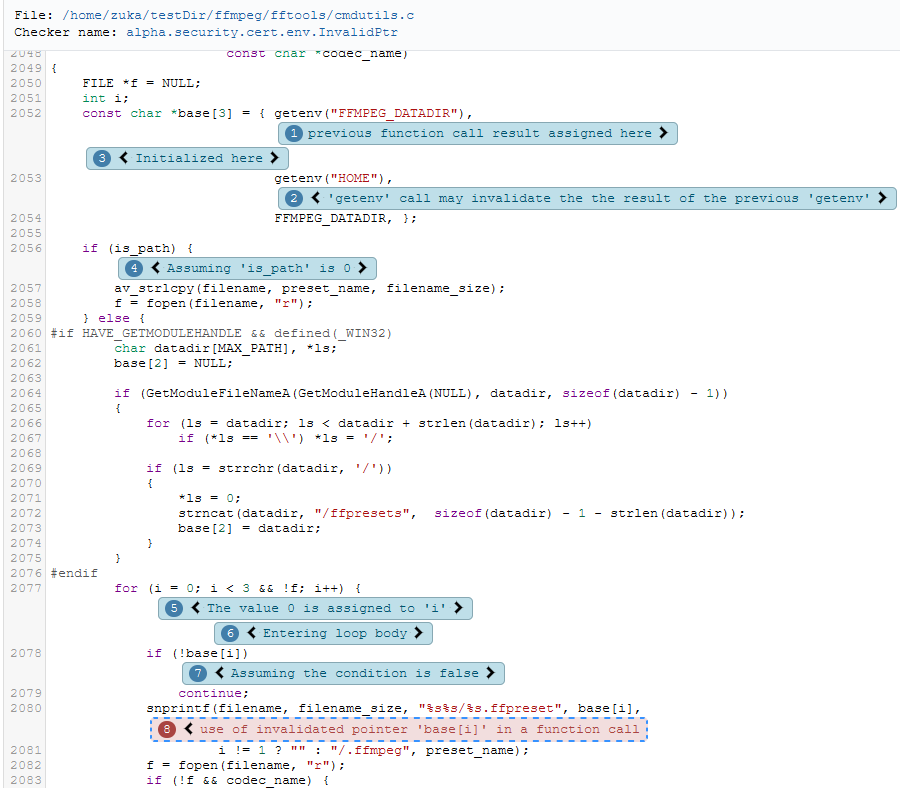
\includegraphics[width=\textwidth]{images/ffmpeg.png}
	\caption{Invalidated pointer usage in FFmpeg}
	\label{fig:ffmpeg-rep}
\end{figure}

\begin{figure}[H]
	\centering
	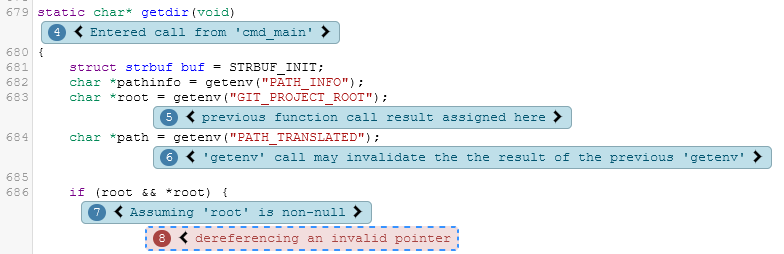
\includegraphics[width=\textwidth]{images/git_report.PNG}
	\caption{Invalidated pointer dereference in Git}
	\label{fig:git-rep}
\end{figure}
